\subsection{%
  Виды векторных полей и их свойства (теоремы о поле градиента и поле вихря).%
}

\begin{definition}
  Если \(\rot \vec{F} = 0\), то поле \(\vec{F}\) называется безвихревым.
\end{definition}

\begin{definition}
  Если \(\div \vec{F} = 0\), то поле \(\vec{F}\) называется соленоидальным.
\end{definition}

\begin{twocolumns}
  \begin{figure}[H]
  \centering

  \begin{subfigure}[b]{0.2\textwidth}
    \centering
    
    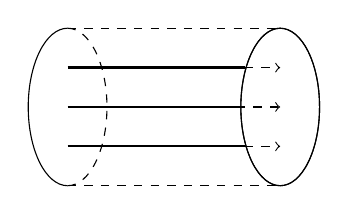
\begin{tikzpicture}
  \draw (0, 1) arc (90 : 270 : 0.5 and 1);
  \draw[dashed] (0, -1) arc (-90 : 90 : 0.5 and 1);

  \draw[thick] (0, -0.5) -- (2.25, -0.5);
  \draw[dashed, ->] (2.25, -0.5) -- (2.7, -0.5);

  \draw[thick] (0, 0) -- (2.15, 0);
  \draw[dashed, ->] (2.15, 0) -- (2.7, 0);

  \draw[thick] (0, 0.5) -- (2.25, 0.5);
  \draw[dashed, ->] (2.25, 0.5) -- (2.7, 0.5);

  \draw (2.7, 0) ellipse (0.5 and 1);
  \draw (2.7, 0) ellipse (0.5 and 1);

  \draw[dashed] (0, 1) -- (2.7, 1);
  \draw[dashed] (0, -1) -- (2.7, -1);
\end{tikzpicture}

    \caption{\(\rot \vec{F} = 0\)}\label{fig:curl}

  \end{subfigure}
  \qquad
  \begin{subfigure}[b]{0.2\textwidth}
    \centering

    \begin{tikzpicture}[
  decoration = {
    markings,
    mark = between positions 0.1 and 1 step 30pt with
      {\arrow[line width = 1pt]{>}}
  }
] 
  \foreach \h in {0, 1, 2} {
    \draw[postaction = { decorate }] (0, \h) ellipse (1 and 0.3);
  };
  \draw[dashed] (-1, 0) -- (-1, 2);
  \draw[dashed] (1, 0) -- (1, 2);
\end{tikzpicture}

    \caption{\(\div \vec{F} = 0\)}\label{fig:solenoidal}

  \end{subfigure}
\end{figure}

  \columnbreak

  \begin{remark}
    Безвихревому полю соответствуют незамкнутые векторные линии, а
    соленоидальному~--- замкнутые.
  \end{remark}
\end{twocolumns}

\begin{remark}
  В действительности поле может быть сложнее, но можно показать, что всякое поле
  является композицией этих двух типов.
\end{remark}

\begin{definition}
  Векторное поле \(\vec{F}\) называется потенциальным, если

  \begin{align*}
    \exists u(x, y, z) \colon \vec{F} = \grad u
  \end{align*}

  Функция \(u(x, y, z)\) в этом случае называется скалярным потенциалом поля
  \(\vec{F}\).
\end{definition}

\begin{theorem}\label{potential-field}
  Всякое безвихревое потенциально. Другими словами

  \begin{align*}
    \rot \vec{F} = 0 \iff \exists u(x, y, z) \colon \vec{F} = \grad u
  \end{align*}
\end{theorem}
\begin{proof}
  \(\implies\) По определению ротора (в координатной форме):

  \begin{align*}
    \rot \vec{F} =
    \left(\frac{\partial R}{\partial y} - \frac{\partial Q}{\partial z}\right)
      \vec{i} +
    \left(\frac{\partial P}{\partial z} - \frac{\partial R}{\partial x}\right)
      \vec{j} +
    \left(\frac{\partial Q}{\partial x} - \frac{\partial P}{\partial y}\right)
      \vec{k}
    = 0
    \\
    \frac{\partial R}{\partial y} = \frac{\partial Q}{\partial z}
    \qquad
    \frac{\partial P}{\partial z} = \frac{\partial R}{\partial x}
    \qquad
    \frac{\partial Q}{\partial x} = \frac{\partial P}{\partial y}
  \end{align*}

  Подберем \(u(x, y, z)\) так, чтобы \(u'_{x} = P\), \(u'_{y} = Q\) и
  \(u'_{z} = R\). Тогда:

  \begin{align*}
    \frac{\partial R}{\partial y}
    = \frac{\partial^2 u}{\partial y \partial z} 
    = \frac{\partial Q}{\partial z}
  \end{align*}

  \(\impliedby\) Пусть \(\exists u(x, y, z) \colon \vec{F} = \grad u\).
  Тогда по определению ротора (в векторной форме):

  \begin{align*}
    \rot \vec{F}
    = \rot \grad u
    = \grad \times \grad \cdot u
    = \under{(\grad \times \grad)}{\text{= 0}} \cdot u
    = 0
  \end{align*}
\end{proof}

\begin{corollary}
  \begin{align*}
    \rot \grad u = 0
  \end{align*}
\end{corollary}

\begin{theorem}
  \begin{align*}
    \div \rot \vec{F} = 0
  \end{align*}
\end{theorem}
\begin{proof}
  По определению дивергенции и ротора (в векторной форме)

  \begin{align*}
    \div \rot \vec{F}
    = \grad \cdot (\grad \times \vec{F})
    = \under{(\grad \times \grad)}{\text{= 0 }} \cdot \vec{F}
    = 0
  \end{align*}
\end{proof}
